\documentclass[10pt]{article}
\usepackage[margin=0.85in]{geometry}
\usepackage[T1]{fontenc}\usepackage{courier}
\usepackage{mathptmx}
\usepackage{amsmath,amssymb}
\usepackage{graphicx,booktabs,multirow,tabularx}
\usepackage[font=small,labelfont=bf]{caption}
\usepackage{enumitem}
\usepackage[hidelinks]{hyperref}
\setlist{nosep,leftmargin=1.3em}
\setlength{\parskip}{3pt}
\setlength{\parindent}{0pt}
\newcommand{\pt}{\,pt}

\title{\vspace{-1.2em}\textbf{Distilling Large Teachers into a 4.9M-Parameter ResNet for CIFAR-10}\\[2pt]
\large Deep Learning (Fall 2026), Project 1}
\author{Rahim Askarov (ra3716) \qquad Philip Vetsas (pmv264)\\[2pt]
NYU Tandon School of Engineering\\[3pt]
\normalsize Code: \url{https://github.com/RoroDev2023/nyu-dl-f26-challenge}}
\date{}

\begin{document}
\maketitle
\vspace{-2.2em}

\section*{Overview}
The task was to design a residual network \cite{he2016deep} with at most 5 million trainable parameters,
trained from scratch on the competition's version of the CIFAR-10 training set \cite{krizhevsky2009} (50,000 images),
and to maximize accuracy on a hidden 2,000-image test set. Our final model, \texttt{r3\_80\_2-3-3}, is a
three-stage ResNet with 80/160/256 channels and 2/3/3 basic blocks
(\textbf{4,880,474 parameters}). It is trained for 1,200 epochs with SGD, strong augmentation,
sharpness-aware minimization (SAM), an exponential moving average (EMA) of the weights, and
knowledge distillation (KD) from three much larger teachers that we trained ourselves on the same
data. At test time we average the softmax of 10 shifted and flipped views.

\textbf{Summary of findings.}
\begin{itemize}
\item \textbf{Final result}: \textbf{91.1\% on the Kaggle public leaderboard}; on our fixed 5,000-image
  validation holdout the same recipe reaches \textbf{97.92\%} (600 epochs). A plain ResNet of the same
  size reaches 95.42\%.
\item Most of the gain came from the training recipe, not the architecture: augmentation + SAM + EMA
  gave +1.9\pt, distillation +0.4\pt, a better width/depth split +0.1--0.2\pt, test-time augmentation
  (TTA) +0.1\pt.
\item With a fixed budget, a middle ground between depth and width won: 80/160/256 channels with
  8 blocks beat a deeper (11 blocks, 64--256 channels) and a wider (6 blocks, 96--320 channels) variant.
\item Many published tricks did not help on top of this recipe when tested against a matched control:
  stochastic depth ($-$18 images, $p{=}.005$), SWA, weight soups, logit-standardized KD,
  test-time BN adaptation, AugMix, and splitting the budget into a two-model ensemble.
\item Validation accuracy (97.9\%) is far above the test score (91.1\%). We verified the pipeline end to end
  (the notebook reproduces the submitted file label for label); the remaining gap looks like a
  distribution shift between the training data and the hidden test images (Section~\ref{sec:gap}).
\end{itemize}

\section{Methodology}

\subsection{Data and evaluation protocol}
We hold out a fixed, class-balanced validation set of 5,000 training images
(\texttt{train\_val\_split(val\_size=5000, seed=0)}). Every student \emph{and every teacher} holds out
the same images, so no teacher has seen a validation image. Models are compared on these 5,000 images with a
\emph{paired} test: for two models we count the images only one of them gets right and apply an exact
two-sided sign test. One validation image is 0.02\pt, and differences below about 8--10 images
were usually noise in repeated runs. We reuse the same validation set many times, so the p-values are
exploratory. The final submission is retrained on all 50,000 images with the chosen recipe.
Since that run has no holdout, we report the validation numbers of the identical 600-epoch run (A4).

\subsection{Architecture}
We keep the residual block exactly as specified: $\mathrm{ReLU}(S(x)+F(x))$ with
$F$ = conv$\to$BN$\to$ReLU$\to$conv$\to$BN, and look for the best split of the 5M budget over the design
variables of the assignment:
number of stages $N$, blocks per stage $B_i$, channels $C_i$, conv kernel $F_i$, shortcut kernel $K_i$, and pool size $P$.

\begin{itemize}
\item \textbf{Stem and pooling.} A 3$\times$3 conv stem without max-pooling keeps the full 32$\times$32 resolution in
  stage 1, which matters for 32-pixel images. The head is global average pooling ($P{=}8$, the final 8$\times$8
  map) followed by one linear layer.
\item \textbf{Kernels.} $F_i{=}3$ everywhere. A 5$\times$5 kernel costs 2.8$\times$ the parameters of a 3$\times$3 one,
  and two stacked 3$\times$3 convs already cover a 5$\times$5 receptive field. The shortcut is the identity inside a stage,
  and a 1$\times$1 conv + BN with stride 2 ($K_i{=}1$) when the resolution halves. A 3$\times$3 shortcut would only spend budget
  on a path whose job is to pass information through.
\item \textbf{Depth vs width.} The number of parameters of a stage grows with $B_i C_i^2$, so with a fixed budget there is a direct trade-off
  between depth and width. Table~\ref{tab:arch} lists the candidates (all 4.7--4.9M parameters).
  Three stages with 8 blocks of 80--256 channels won the 300-epoch sweep. Very deep, narrow nets (24 blocks of
  40--160 channels) and a fourth stage at 4$\times$4 resolution were slower per epoch and could not be
  finished within our compute; we dropped them.
\item \textbf{Initialization.} He initialization; the last BN of each block starts at zero, so every block begins as
  the identity \cite{goyal2017}, which made the 1,200-epoch runs stable from the first epoch.
\end{itemize}

\begin{table}[t]
\centering\small
\caption{Student architectures (all 3$\times$3 convs, 1$\times$1 projection shortcuts, global average pool).
Validation = 300 epochs, identical recipe with KD from 3 teachers, EMA weights, flip TTA.}
\label{tab:arch}
\begin{tabular}{llrrc}
\toprule
Name & Channels $C_i$ / blocks $B_i$ & Params & Val (\%) & Notes\\
\midrule
\textbf{r3\_80\_2-3-3} & 80, 160, 256 / 2, 3, 3 & 4,880,474 & \textbf{97.62} & chosen\\
r3\_96\_2-2-2 & 96, 192, 320 / 2, 2, 2 & 4,902,506 & 97.42 & widest, shallowest\\
r3\_64\_3-5-3 & 64, 128, 256 / 3, 5, 3 & 4,918,602 & 97.38 & first design\\
r4\_64\_3-3-2-1 & 64, 128, 256, 320 / 3, 3, 2, 1 & 4,890,442 & -- & not finished\\
r3\_40\_8-8-8 & 40, 80, 160 / 8, 8, 8 & 4,722,610 & -- & not finished (slow)\\
\midrule
WRN-40-2 ($\times$2 ensemble) & 32, 64, 128 / 6, 6, 6 (pre-act) & 2$\times$2,243,546 & 97.26 & both together\\
\bottomrule
\end{tabular}
\end{table}

\textbf{Pros and cons.} Wider stages give each block more features to work with and run faster on a
GPU (fewer sequential layers), but every extra block is expensive. Deeper nets reuse parameters over more
nonlinear steps but are slower and, at this size, become too narrow early on (40 channels at full
resolution). Spending more width at low resolution (r3\_96, 320 channels in stage 3) was worse than
r3\_80, which moves capacity to the 16$\times$16 stage. Our reading is that mid-resolution features matter
most for 32$\times$32 objects.

\subsection{Training recipe}
All models use SGD with Nesterov momentum 0.9, batch 128, peak learning rate 0.1 with 5 warmup epochs and
per-step cosine decay to 0 \cite{loshchilov2017sgdr}, and weight decay $5\cdot10^{-4}$ (not on BN parameters or biases). Mixed precision
(bf16) is used on A100/H100 GPUs. On top of random crop (4\,px padding) + horizontal flip we add:
\begin{itemize}
\item \textbf{TrivialAugment} \cite{muller2021trivial} (one random photometric/geometric op per image, random strength) and
  \textbf{Cutout} 16$\times$16 \cite{devries2017cutout}.
\item \textbf{mixup} ($\alpha{=}0.2$) \cite{zhang2018mixup} or \textbf{CutMix} ($\alpha{=}1$) \cite{yun2019cutmix}, chosen at random per batch,
  turned off for the final 50 of 1,200 epochs (15 of 300) so the model ends on clean images.
\item \textbf{SAM} \cite{foret2021sam} with $\rho{=}0.05$: each step first moves the weights in the direction that increases the loss most
  (inside a small ball), and then takes the gradient there. This costs a second forward/backward pass. BN running
  statistics from the perturbed pass are discarded.
\item \textbf{EMA} of the weights with decay 0.999; we evaluate and submit the EMA weights.
\item Label smoothing 0.1 \cite{szegedy2016rethinking}, only when there are no teachers (with KD the soft targets already do this).
\end{itemize}

\subsection{Knowledge distillation}
A 5M-parameter model trained on 50k images is limited mostly by how much the labels can teach it, not by
optimization. Following \cite{hinton2015distilling}, we first train large teachers from scratch on the same 45k training images
with the same recipe (400 epochs): two \textbf{WRN-28-10} \cite{zagoruyko2016wide} (36.5M parameters, val 98.06\% and 98.12\%)
and a \textbf{PyramidNet-110} ($\alpha{=}270$) with ShakeDrop \cite{han2017pyramidal,yamada2019shakedrop} (28.5M, 97.64\%).
The teachers are only used during training. At inference the system is the single 4.88M student.

The student loss is
\[
\mathcal{L} = (1-\alpha)\,\mathrm{CE}(z_s, y) + \alpha\,T^2\,\mathrm{KL}\!\left(\bar p_T \,\|\, \mathrm{softmax}(z_s/T)\right),\qquad
\bar p_T = \tfrac{1}{3}\textstyle\sum_k \mathrm{softmax}(z_k/T),
\]
with $\alpha{=}0.9$ and $T{=}4$. A key detail is \emph{consistent teaching} \cite{beyer2022patient}: the teachers see exactly the same augmented, mixed batch as the
student (instead of clean images), so the soft targets describe the image the student actually sees. Together with
heavy augmentation, this lets distillation benefit from very long schedules. Going from 600 to 1,200 epochs did not hurt
on validation (97.92 vs 97.94\%), and the longer schedule gave our best test score.

\subsection{Test-time augmentation}
We reflect-pad each test image by 4 pixels and take five 32$\times$32 windows (centered and shifted by $\pm$2 pixels
vertically or horizontally), plus the same five windows of the mirrored image, and average the 10 softmax
outputs. This adds no parameters. On validation it adds +0.08\pt\ over flip-only TTA. Weighting the center views
more (50\% or 80\% of the weight) or adding diagonal shifts did not help when tuned on one half of
validation and checked on the other.

\subsection{Compute}
Training ran on NYU HPC (A100), Modal and Vast.ai (A100/H100). With KD from three teachers and SAM, one
epoch of the student takes 27\,s on an A100 (18\,s on an H100 with GPU-side augmentation). The final
1,200-epoch run took about 9 GPU-hours, and each WRN-28-10 teacher about 3 GPU-hours.

\section{Results}

\subsection{Final model}
\begin{table}[h]
\centering\small
\caption{Final submission. ``Val'' uses the identical recipe at 600 epochs with the 5,000-image holdout (A4).}
\label{tab:final}
\begin{tabular}{ll}
\toprule
Architecture & ResNet \texttt{r3\_80\_2-3-3}: 3$\times$3 stem (80 ch); stages of 2, 3, 3 basic blocks with 80, 160, 256 channels\\
& at 32$^2$, 16$^2$, 8$^2$ resolution; 1$\times$1 projection shortcuts; global average pool; linear 256$\to$10\\
Parameters & \textbf{4,880,474} trainable (budget 5,000,000; teachers not used at inference)\\
Training & 1,200 epochs on all 50k images, seed 1; KD from 3 teachers; TA, Cutout, mixup/CutMix, SAM, EMA\\
Inference & EMA weights, 10-view TTA (5 shifts $\times$ flip), softmax average\\
Validation accuracy & \textbf{97.92\%} (no TTA 97.72\%, flip TTA 97.84\%)\\
\textbf{Test accuracy} & \textbf{91.1\%} (Kaggle public leaderboard)\\
\bottomrule
\end{tabular}
\end{table}

\begin{figure}[t]
\centering
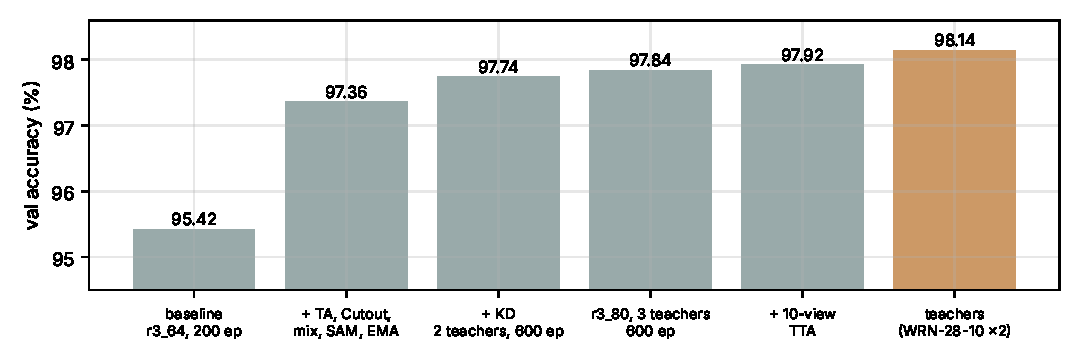
\includegraphics[width=\linewidth]{../figures/steps.pdf}
\vspace{-1.5em}
\caption{Validation accuracy as components are added (EMA weights; student bars use flip TTA except the 10-view TTA bar).
The last bar is the best teacher pair (two WRN-28-10, 73M parameters), which bounds what distillation can reach.}
\label{fig:steps}
\end{figure}

\begin{figure}[t]
\centering
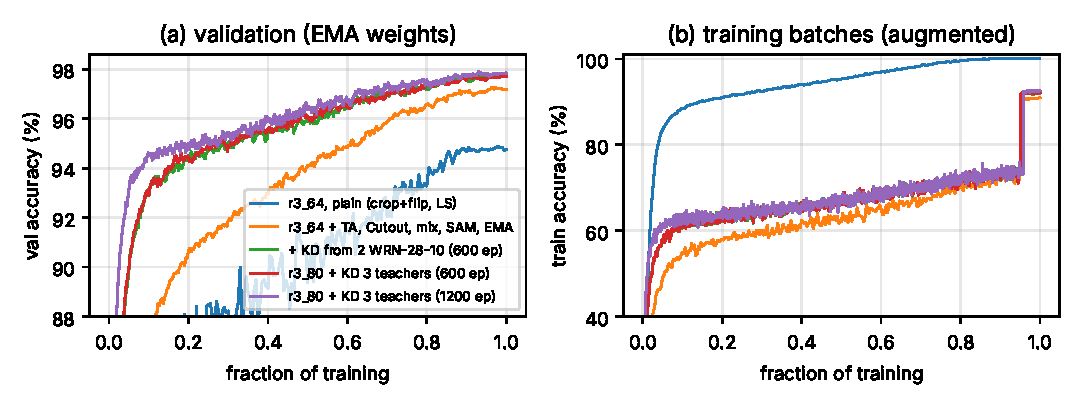
\includegraphics[width=\linewidth]{../figures/curves.pdf}
\vspace{-1.5em}
\caption{(a) Validation accuracy during training (x axis normalized, runs are 200--1,200 epochs). Strong augmentation
makes early validation accuracy worse, but the final accuracy much better. (b) Training accuracy on augmented, mixed batches stays at 60--75\% while mixing is on
and only reaches about 92\% after it is turned off near the end; the plain baseline memorizes its training set (100\%).}
\label{fig:curves}
\end{figure}

\subsection{Contribution of each component}
Figure~\ref{fig:steps} breaks the result down. The plain baseline (\texttt{r3\_64\_3-5-3}, crop + flip, label smoothing, 200 epochs)
reaches 95.42\%. The augmentation + SAM + EMA recipe adds +1.9\pt, distillation from two WRN teachers with a 600-epoch schedule
+0.4\pt, the r3\_80 architecture with three teachers +0.1\pt, and 10-view TTA +0.08\pt. The student ends 0.2\pt\ below its
teachers, which have 15$\times$ more parameters. Figure~\ref{fig:curves} shows that the baseline fits its training set perfectly while the
regularized models never do. This is the main reason long schedules keep helping instead of overfitting.

\subsection{What did not help}
We judged every idea against a matched control (same start point or same seed and recipe, one change) on the same validation images.
Figure~\ref{fig:ablations} shows the controlled comparisons. Table~\ref{tab:neg} lists the rest.

\begin{figure}[t]
\centering
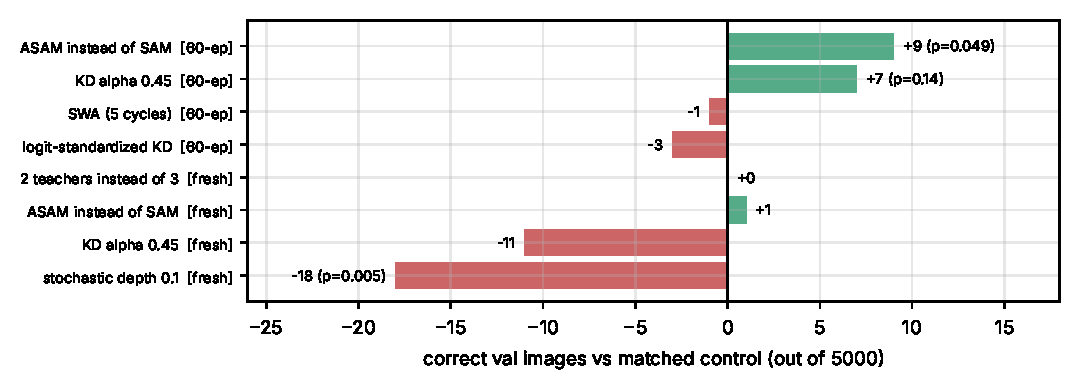
\includegraphics[width=\linewidth]{../figures/ablations.pdf}
\vspace{-1.5em}
\caption{Paired differences against a matched control, in correctly classified validation images (out of 5,000; 5 images = 0.1\pt).
``60-ep'' = 60-epoch continuation of A4 (control: SAM continuation); ``fresh'' = 300-epoch run from scratch.}
\label{fig:ablations}
\end{figure}

\begin{table}[t]
\centering\small
\caption{Other experiments. Accuracy on validation (10-view TTA, EMA) unless marked as public leaderboard (LB).}
\label{tab:neg}
\begin{tabularx}{\linewidth}{lX}
\toprule
Experiment & Result\\
\midrule
ASAM \cite{kwon2021asam} instead of SAM & +9 images as a 60-epoch continuation ($p{=}.049$), confirmed weakly from a second start point (+1/+4),
but no continuation beat its \emph{untouched} start model. From scratch (300 ep): +1 image. On the test set, ASAM finish of F2s1: LB 0.908 vs 0.911.\\
Stochastic depth 0.1 \cite{huang2016deep} & $-$18 images ($p{=}.005$) and worse calibration: on top of KD + SAM + mixing, extra regularization hurts.\\
SWA \cite{izmailov2018swa} & 6 cyclic 10-epoch cycles, averaged, BN recomputed: $-$1 image vs control, $-$6 vs start.\\
Weight soup \cite{wortsman2022soups} & Average of a model and its fine-tuned version: $-$1/$-$3 images; on test 0.908.\\
Logit-standardized KD \cite{sun2024logit} & Same accuracy as ordinary KD (97.62 vs 97.62, 300 ep), much better calibration (val NLL 0.09 vs 0.15).\\
KD $\alpha{=}0.45$; 2 vs 3 teachers & $\alpha{=}0.45$: $-$11 images from scratch. Dropping the PyramidNet teacher: $\pm$0.\\
Two WRN-40-2 (ensemble) & 2.24M each, 97.10/97.06 alone, 97.26 averaged vs 97.62 for one 4.88M ResNet: one model is better than two half-size models.\\
AugMix + JSD \cite{hendrycks2020augmix} & 80-ep finish: +0.6\pt\ on blurred validation images but $-$0.6\pt\ on clean images.\\
Test-time BN adaptation & Re-estimating BN statistics on the test images: val 97.34, LB 0.884 (worse). BN recalibration on clean train images: $-$0.6 to $-$0.8\pt.\\
Class-balanced prediction & Sinkhorn balancing \cite{cuturi2013sinkhorn} of the test predictions: LB 0.898 vs 0.899.\\
More epochs & 600$\to$1,200 epochs: 97.92$\to$97.94 (+1 image). A random seed changes 61/2000 test labels and up to 1.3\pt\ on the LB.\\
\bottomrule
\end{tabularx}
\end{table}

\subsection{Validation vs.\ test gap}\label{sec:gap}
Our validation accuracy (97.9\%) is about 7\pt\ above the public test score (91.1\%). We checked the obvious causes:
no overlap between training and validation images; the exact submission code gives 97.82\% on validation;
the notebook regenerates the submitted CSV with 0 differing labels; per-class validation accuracy is unremarkable.
What we did measure is that the test images differ from the training images: they are brighter
(mean RGB 0.513/0.498/0.461 vs 0.491/0.482/0.447), have higher contrast, are about 7\% sharper and less saturated.
The student is less confident on test (0.85 vs 0.90 mean max-probability) and agrees less with its teachers (96.9\% vs 99.2\%).
However, simulating these pixel statistics on validation costs only 0.1--0.3\pt. Our hypothesis, which we could not test without
test labels, is a content-level shift like CIFAR-10.1 \cite{recht2018cifar}, where re-collected test images cost CIFAR-10 models
4--10\pt. A consequence is that public LB differences of about $\pm$0.5\pt\ between runs were mostly noise (2,000 images,
seed variance), so we made decisions on the paired validation tests and used the leaderboard only as a final check.

\section{Lessons learned}
\begin{itemize}
\item \textbf{The recipe matters more than the architecture.} Among sensible 5M ResNets the spread was 0.25\pt.
  Augmentation, SAM, EMA and distillation together were worth about 2.3\pt.
\item \textbf{Distillation needs strong, matching teachers.} Teachers trained with the same augmentation, fed the student's own
  augmented batch, made long schedules (600--1,200 epochs) useful for a small model.
\item \textbf{Do not stack regularizers blindly.} Once the model is strongly regularized (it never fits its training set),
  stochastic depth, AugMix and lower KD weight all hurt.
\item \textbf{Test against a matched control.} Many ideas looked good against an earlier, different baseline and disappeared in a paired comparison.
  Late ``finishing'' runs from a converged checkpoint never improved on the checkpoint itself.
\item \textbf{One budget, one model.} Two half-size models averaged lost 0.36\pt\ to one full-size model.
\item \textbf{Be careful with a small public test set.} With 2,000 test images and a shifted distribution, seed noise on the
  leaderboard is as large as most real improvements.
\end{itemize}

\section*{Code}
The repository contains the training code (\texttt{train.py}, all tricks as flags), models (\texttt{models.py}), KD/SAM/EMA/mixing
(\texttt{tricks.py}), the single TTA implementation (\texttt{tta.py}), evaluation scripts, the per-run logs and arguments
(\texttt{runs/}), a full experiment log (\texttt{EXPERIMENTS.md}), and \texttt{report.ipynb}, which prints the parameter count,
reproduces the submission and the validation accuracy, and makes every figure in this report.
Parts of our setup (no max-pool stem for 32$\times$32 inputs, standard CIFAR training pipeline) follow common practice as in
\cite{kuangliu}. Teacher architectures follow the original papers.

\small
\begin{thebibliography}{99}\setlength{\itemsep}{0pt}
\bibitem{he2016deep} K.~He, X.~Zhang, S.~Ren, J.~Sun. Deep residual learning for image recognition. CVPR 2016.
\bibitem{krizhevsky2009} A.~Krizhevsky. Learning multiple layers of features from tiny images. Tech.\ report, 2009.
\bibitem{goyal2017} P.~Goyal et al. Accurate, large minibatch SGD: training ImageNet in 1 hour. arXiv:1706.02677, 2017.
\bibitem{loshchilov2017sgdr} I.~Loshchilov, F.~Hutter. SGDR: stochastic gradient descent with warm restarts. ICLR 2017.
\bibitem{muller2021trivial} S.~M\"uller, F.~Hutter. TrivialAugment: tuning-free yet state-of-the-art data augmentation. ICCV 2021.
\bibitem{devries2017cutout} T.~DeVries, G.~Taylor. Improved regularization of CNNs with Cutout. arXiv:1708.04552, 2017.
\bibitem{zhang2018mixup} H.~Zhang, M.~Cisse, Y.~Dauphin, D.~Lopez-Paz. mixup: beyond empirical risk minimization. ICLR 2018.
\bibitem{yun2019cutmix} S.~Yun et al. CutMix: regularization strategy to train strong classifiers with localizable features. ICCV 2019.
\bibitem{foret2021sam} P.~Foret, A.~Kleiner, H.~Mobahi, B.~Neyshabur. Sharpness-aware minimization for efficiently improving generalization. ICLR 2021.
\bibitem{kwon2021asam} J.~Kwon, J.~Kim, H.~Park, I.~Choi. ASAM: adaptive sharpness-aware minimization. ICML 2021.
\bibitem{szegedy2016rethinking} C.~Szegedy et al. Rethinking the Inception architecture for computer vision. CVPR 2016.
\bibitem{hinton2015distilling} G.~Hinton, O.~Vinyals, J.~Dean. Distilling the knowledge in a neural network. arXiv:1503.02531, 2015.
\bibitem{beyer2022patient} L.~Beyer et al. Knowledge distillation: a good teacher is patient and consistent. CVPR 2022.
\bibitem{sun2024logit} S.~Sun et al. Logit standardization in knowledge distillation. CVPR 2024.
\bibitem{zagoruyko2016wide} S.~Zagoruyko, N.~Komodakis. Wide residual networks. BMVC 2016.
\bibitem{han2017pyramidal} D.~Han, J.~Kim, J.~Kim. Deep pyramidal residual networks. CVPR 2017.
\bibitem{yamada2019shakedrop} Y.~Yamada et al. ShakeDrop regularization for deep residual learning. IEEE Access, 2019.
\bibitem{huang2016deep} G.~Huang et al. Deep networks with stochastic depth. ECCV 2016.
\bibitem{izmailov2018swa} P.~Izmailov et al. Averaging weights leads to wider optima and better generalization. UAI 2018.
\bibitem{wortsman2022soups} M.~Wortsman et al. Model soups: averaging weights of multiple fine-tuned models improves accuracy. ICML 2022.
\bibitem{hendrycks2020augmix} D.~Hendrycks et al. AugMix: a simple data processing method to improve robustness and uncertainty. ICLR 2020.
\bibitem{cuturi2013sinkhorn} M.~Cuturi. Sinkhorn distances: lightspeed computation of optimal transport. NeurIPS 2013.
\bibitem{recht2018cifar} B.~Recht, R.~Roelofs, L.~Schmidt, V.~Shankar. Do CIFAR-10 classifiers generalize to CIFAR-10? arXiv:1806.00451, 2018.
\bibitem{kuangliu} K.~Liu. pytorch-cifar: 95.47\% on CIFAR-10 with PyTorch. \url{https://github.com/kuangliu/pytorch-cifar}.
\end{thebibliography}
\end{document}
